\documentclass[10pt]{beamer} % die 10pt sollten festgelegt bleiben, da dies die Groesse der Mathematikschrift etc. beeinflusst
\usepackage[ngerman]{babel}  % deutsche Bezeichnungen und Trennung etc
\usepackage{hyperref}        % interne Hyperlinks
\usepackage[mnf,footuni, headframelogo]{./unirostock/beamerthemeRostock}
\usepackage[utf8]{inputenc}
\usepackage{amsmath}
\usepackage{amssymb}
\usepackage{mathtools}

%cmd
\newcommand{\ol}{\overline} %Kurzform für \overline definiert 
\newcommand{\olsi}[1]{\,\overline{\!{#1}}} % overline short italic
\newcommand{\ols}[1]{\mskip.5\thinmuskip\overline{\mskip-.5\thinmuskip {#1} \mskip-.5\thinmuskip}\mskip.5\thinmuskip} % overline short

%\hyphenation{Online-Back-pro-pa-ga-tions-algo-rithmus Online-Backpropagationsalgorithmus}



%\newcommand{\RR}{\mathbb{R}}
%newcommand{\RRn}{\mathbb{R}^n}

\newcommand{\RR}{\ensuremath{\mathbb{R}}}
\newcommand{\Rnv}{\ensuremath{\mathbb{R}^{n}}}
\newcommand{\Rnn}{\ensuremath{\mathbb{R}^{n\times n}}}

\newcommand{\NN}{\ensuremath{\mathbb{N}}}

\newcommand{\mK}{\ensuremath{\mathcal{K}}}
\newcommand{\mKp}{\ensuremath{\mathcal{K}}^+}
\newcommand{\Code}{\ensuremath{C^{\textnormal{dgl}}}}


%%%%


%%%%%%%%%%%% Festlegung der Titelseite %%%%%%%%%%%%%%%%%%%%%%%%%%%%%%%%%
\title[Datenbankgestützte Erkennung von Mustern in trainierten gefalteten neuronalen Netzen]{Datenbankgestützte Erkennung von Mustern in trainierten gefalteten neuronalen Netzen}

\subtitle{Verteidigung}

\author{\textsc{Florian Baldauf}}

\date{14. September 2022}

\institute{Universität Rostock, Institut für Mathematik}

\footinstitute{Mathematisch Naturwissenschaftliche Fakultät, Institut für Mathematik}

\renewcommand{\mylogo}{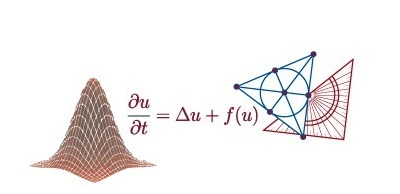
\includegraphics[height=15mm]{institut}}


%%%%%%%%%%%%%%%%%% Los geht's %%%%%%%%%%%%%%%%%%%%%%%%%%%%%%%%%%%%%%%%%
%%%%%%%%%%%%%%%%%%%%%%%%%%%%%%%%%%%%%%%%%%%%%%%%%%%%%%%%%%%%%%%%%%%%%%%
\begin{document}


%%%%%%%%%%%%%%%%%%%%%%%%%%%%%%%%%%%%%%%%%%%%%%%%%%%%%%%%%%%%%%%%%%%%%%%
%%%%%%%%%%%%%%%%%%%%%%%%%%%%%%%%%%%%%%%%%%%%%%%%%%%%%%%%%%%%%%%%%%%%%%%
\begin{frame}% Titelseite
  \titlepage
\end{frame}


%%%%%%%%%%%%%%%%%%%%%%%%%%%%%%%%%%%%%%%%%%%%%%%%%%%%%%%%%%%%%%%%%%%%%%%
%%%%%%%%%%%%%%%%%%%%%%%%%%%%%%%%%%%%%%%%%%%%%%%%%%%%%%%%%%%%%%%%%%%%%%%
\begin{frame}{Struktur der Vortrages}%{Damit der Hörer auch ein wenig durchsieht}
  \tableofcontents[pausesections]
\end{frame}


%%%%%%%%%%%%%%%%%%%%%%%%%%%%%%%%%%%%%%%%%%%%%%%%%%%%%%%%%%%%%%%%%%%%%%%
%%%%%%%%%%%%%%%%%%%%%%%%%%%%%%%%%%%%%%%%%%%%%%%%%%%%%%%%%%%%%%%%%%%%%%%
\section{Einführung Mathematik und Künstlichen Intelligenz}

\begin{frame}
   \frametitle{KI im öffentlichen Leben} % Dieses Frame wird je nach Platz/Inhalt/Fuellstand automatisch geteilt
%\begin{theorem}
%	Diese Box ist sch\"on.
%\end{theorem}

%\begin{proof}
%	Die CD-Vorlage ist insgesamt schick, ergo muss jedes Teil hiervon dekorativ %sein, folglich also auch die obige Theorem-Box.
%\end{proof}

%\begin{Beispiel}
%	$ \sigma(u,v) \coloneqq a + up + vq $
%\end{Beispiel}

%\begin{block}{Blocktitel}
%	Ein Block mit dem Titel \insertblocktitle
%\end{block}

%\begin{alertblock}{Alertblocktitel}
%	Ein Alertblock.
%\end{alertblock}

%\begin{exampleblock}{Beispielblocktitel}
%	Ein Beispielblock.
%\end{exampleblock}
\end{frame}

\begin{frame}
   \frametitle[]{Erfolg in vielen Disziplinen}
\end{frame}

\begin{frame}
   \frametitle[]{Auswirkungen auf die Mathematik}
   Einige Beispiele:
   \begin{itemize}
      \item Computer Vision
      \begin{itemize}
         \item Segmentierung
         \item Edge Detection
         \item Klassifikation
         \item angewendet z.B. bei der Computertomographie
         \item $\ldots$
      \end{itemize}
      \pause
      \item Numerische Behandlung von partiellen Differentialgleichungen
      \begin{itemize}
         \item Black-Scholes PDE (Finanzmathematik)
         \item Allen-Cahn PDE (Physik)
      \end{itemize}
   \end{itemize}
\end{frame}

\begin{frame}
   \frametitle[]{Aufgaben der Mathematik}
   Mathematik für Künstliche Intelligenz
   \begin{itemize}
      \pause
      \item Entwicklung einer mathematischen Abstraktion
      \item Kann dadurch die Verlässlichkeit überpüft werden?
   \end{itemize}
   \pause
   Künstliche Intelligenz für Mathematik
   \begin{itemize}
      \item Wie kann KI in Bereichen wie Computer Vision, Spracherkennung, PDE etc. vorteilhaft genutzt werden.
   \end{itemize}
\end{frame}

\begin{frame}
   \frametitle[]{Meine Problemstellungen}
   TODO
\end{frame}
%%%%%%%%%%%% Beispielfolie aus dem BeamerUsersguide %%%%%%%%%%%%%%%%%%%
%%%%%%%%%%%%%%%%%%%%%%%%%%%%%%%%%%%%%%%%%%%%%%%%%%%%%%%%%%%%%%%%%%%%%%%
\subsection{Neuronale Netze}

\begin{frame}
  \frametitle{Erste Ansätze}
Ideen von McCulloch und Pitts (1943):
\begin{itemize}
   \item Entwicklung einer algorithmischen Beschreibung des Lernens
   \item menschliche Gehirn als Vorbild $\rightarrow$ das abstrakte Neuron
\end{itemize}
\end{frame}

\begin{frame}
   \frametitle[]{Das Neuron}
   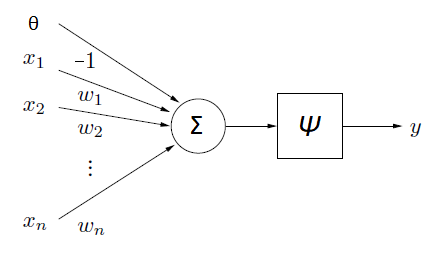
\includegraphics[width=0.9\textwidth]{pics/perzeptron.png}
\end{frame}

\begin{frame}
   \begin{block}{Definition Neuron}
      \label{def_neuron}
      Für eine gegebene Funktion $\phi: \RR \rightarrow \RR$, einen Vektor $w \in \Rnv$ und ein Skalar $b \in \RR$ wird die Funktion 
      \[ \
      \Phi: \RR^n \rightarrow \RR, \; \; \; x \mapsto \phi(w^T x -b)=:y,
      \]
      \textit{Neuron} genannt.
   \end{block}
   \pause
   Mögliche Aktivierungsfunktionen sind:
   \begin{align*}
      \text{Identität}: \; \;\phi(x)&=x, \\
      \text{Logistische Funktion}: \; \;\phi(x)&=\frac{1}{1+\mathrm{e}^{-x}}, \\
      \text{ReLU (rectified linear unit)}: \; \;\phi(x)&=\max\{0,x\}.
  \end{align*}
\end{frame}

\begin{frame}
   Die Verknüpfung von Neuronen zu Netzen führt zur Komposition von affin linearen Abbildungen und Aktivierungsfunktionen.
   \pause

   Ein Beispiel(Quelle Gitta Kutyniok \cite{})
   \begin{equation*}
      \Phi: \RR^3 \rightarrow \RR^2, \; \; \Phi(x)=W^{(2)}\phi(W^{(1)}x-b^{(1)})-b^{(2)}
   \end{equation*}
   
   \begin{minipage}[c]{0.35\textwidth}
      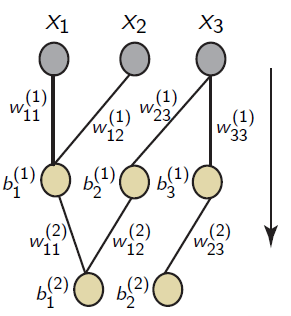
\includegraphics[width=\textwidth]{pics/FF_sparse.png}
      \end{minipage}
      \begin{minipage}[c]{0.3\textwidth}
         \begin{align*}
            W^{(1)} &= \begin{pmatrix}
               w_{11}^{(1)} & w_{12}^{(1)} &0 \\
               0 &0 &w_{23}^{(1)} \\
               0 &0 &w_{33}^{(1)} \\
            \end{pmatrix} \\
            W^{(2)} &= \begin{pmatrix}
               w_{11}^{(2)} & w_{12}^{(1)} &0 \\
               0 &0 &w_{23}^{(2)}
            \end{pmatrix}
         \end{align*}  
      \end{minipage}
\end{frame}

\begin{frame}
   \frametitle[]{Neuronale Netze}
   \begin{block}{Definition Vorwärtsgerichtetes neuronales Netz(FNN)}
      Seien 
      \begin{itemize}
         \item $s_0 \in \mathbb{N}$: Dimension der Eingabeschicht,
         \item $L$: Anzahl der Schichten, 
         \item $\phi$: eine (nichtlineare) Aktivierungsfunktion,
         \item Neuronen: $T_{\ell}: \RR^{s_{\ell-1}} \rightarrow \RR^{s_\ell}, \; \ell=1, \ldots L, \; \text{mit} T_{\ell}(x)=W^{(\ell)}x+b^{(\ell)}$
      \end{itemize}
      \pause
      Dann ist $\Phi: \RR^{s_0} \rightarrow \RR^{s_L}$ durch die Komposition 
      \begin{equation*}
         \Phi(x)=T_{L} \circ \phi \circ T_{L-1} \circ \phi \circ \ldots \circ \phi \circ T_1(x), \; x \in \RR^{s_0}
      \end{equation*}
      erklärt. Der Vektor $y:=\Phi(x)$ wird Ausgabe des (tiefen) FNN genannt.
   \end{block}
\end{frame}

\begin{frame}
   \frametitle[]{Veranschaulichung}
   \begin{figure}
      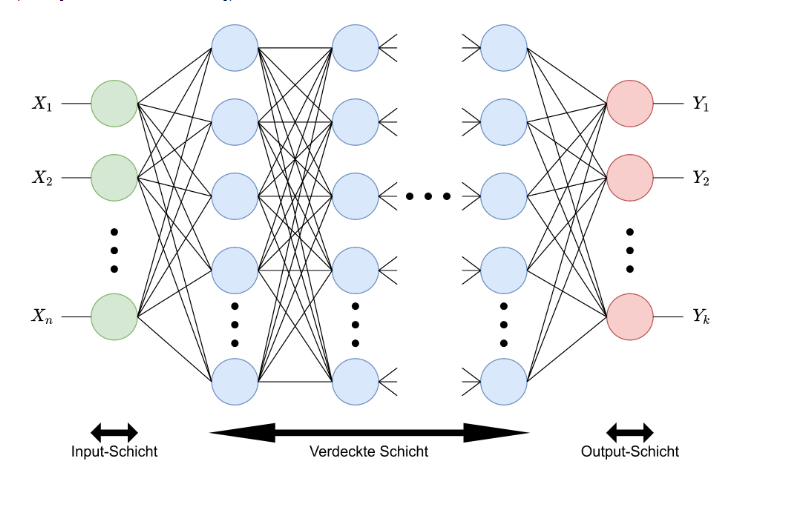
\includegraphics[width=0.8\textwidth]{pics/full_FFN.png}
      \caption[]{Die Abbildung ist aus Fenske\cite[]{fenske} entnommen.}
   \end{figure}
\end{frame}

%%%%%%%%%%%% Beispielfolie zum Mathemodus %%%%%%%%%%%%%%%%%%%%%%%%%%%%%
%%%%%%%%%%%%%%%%%%%%%%%%%%%%%%%%%%%%%%%%%%%%%%%%%%%%%%%%%%%%%%%%%%%%%%%
\subsection{Erkennung von Mustern}
\begin{frame}{Überwachtes Lernen}{Klassifikation von Objekten mithilfe vonFFN}
Gegeben: 
\begin{itemize}
   \item Menge $\mathcal{M}=\{x_i \in \RR^n \, : \, 1 \leq i \leq m\}$,
   \item Funktion $f: \mathcal{M} \rightarrow \{1, \ldots k\}$,
   \item also eine endliche Menge von Tupeln der Form $(x_i, f(x_i))_{i=1}^m$, auch Trainingsmenge $\mathcal{T}$ genannt.
\end{itemize} 
\pause
Gesucht: affin lineare Funktionen $(T_{\ell})_{\ell=1}^L=(W^{(\ell)} \cdot + b^{(\ell)})_{\ell=1}^L$, sodass das Problem

\begin{equation*}
   \underset{(W^{(\ell)}, b^{(\ell)})_\ell}{\min} \sum_{i=1}^m \mathcal{E}(\Phi(x_i),f(x_i)) +\lambda \mathcal{R}((W^{(\ell)}, b^{(\ell)})_l)
\end{equation*}
gelöst wird. Hier ist $\mathcal{E}(\mathcal{T},\mathcal{W})$ eine wählbare Fehlerfunktion.
\end{frame}

\begin{frame}
   \frametitle{Training von FFN}
   Training mithilfe des Gradientenverfahren als iteratives Verfahren mit dem langfristigen Ziel $\Phi(x_i) \approx f(x_i)$ für Testdaten 
   
   $\rightarrow$ Backpropagation
   
   Sei $\mathcal{W}=\{(W^{(\ell)},b^{(\ell)}) \, : \, 1 \leq \ell \leq L\}$ die Menge der Modellparameter.

   Idee: 
   \begin{itemize}
      \pause
      \item Bestimme Gradient $\Delta_n=\nabla_{\mathcal{W}} \mathcal{E}(\mathcal{T},\mathcal{W})$,
      \pause
      \item Aktualisiere Parameter $\mathcal{W}_{n+1}= \mathcal{W}_n+ \lambda \Delta_n$,
      \pause
      \item solange ein Abbruchkriterium nicht erfüllt ist.
   \end{itemize} 

\end{frame}

\begin{frame}
   TODO Bild Rückwärtsrechnung
\end{frame}

%%%%%%%%%%%% Beispielfolie zu  Auzaehlungen %%%%%%%%%%%%%%%%%%%%%%%%%%%
%%%%%%%%%%%%%%%%%%%%%%%%%%%%%%%%%%%%%%%%%%%%%%%%%%%%%%%%%%%%%%%%%%%%%%%
\subsection{Aufz\"ahlungen}
\begin{frame}{Auflistungen und Aufz\"ahlungen}
   Diese Folie hat zur Abwechslung mal keinen Untertitel, daf\"ur ist sie aber zweispaltig.

   \begin{columns}
      \column{0.45\textwidth}
         \begin{itemize}
            \item erster Auflistungspunkt
                  \begin{itemize}
                     \item n\"achste Ebene
                     \item n\"achste Ebene
                           \begin{itemize}
                              \item tiefste Ebene
                              \item tiefste Ebene
                           \end{itemize}
                     \item n\"achste Ebene
                  \end{itemize}
            \item zweiter Auflistungspunkt
         \end{itemize}

      \column{0.45\textwidth}
         \begin{enumerate}
            \item mit Aufz\"ahlungen
                  \begin{enumerate}
                     \item geht das nat\"urlich
                           \begin{enumerate}
                              \item ebenso
                              \item wie mit
                           \end{enumerate}
                     \item Auflistungen
                  \end{enumerate}
         \end{enumerate}
   \end{columns}

\end{frame}


%%%%%%%%%%%% Beispielfolie zu Boxen etc.    %%%%%%%%%%%%%%%%%%%%%%%%%%%
%%%%%%%%%%%%%%%%%%%%%%%%%%%%%%%%%%%%%%%%%%%%%%%%%%%%%%%%%%%%%%%%%%%%%%%
\subsection{Theorem / Beweis / andere Boxen} 

\begin{frame}[allowframebreaks]{Theorem / Beweis / andere Boxen} % Dieses Frame wird je nach Platz/Inhalt/Fuellstand automatisch geteilt
   \begin{theorem}
      Diese Box ist sch\"on.
   \end{theorem}

   \begin{proof}
      Die CD-Vorlage ist insgesamt schick, ergo muss jedes Teil hiervon dekorativ sein, folglich also auch die obige Theorem-Box.
   \end{proof}

   \begin{Beispiel}
     Diese Box ist auch ein nettes Beispiel f\"ur schicke Boxen.
   \end{Beispiel}

   \begin{block}{Blocktitel}
      Ein Block mit dem Titel \insertblocktitle
   \end{block}

   \begin{alertblock}{Alertblocktitel}
      Ein Alertblock.
   \end{alertblock}

   \begin{exampleblock}{Beispielblocktitel}
      Ein Beispielblock.
   \end{exampleblock}

\end{frame}

%%%%%%%%%%%% Details zum Style %%%%%%%%%%%%%%%%%%%%%%%%%%%%%%%%%%%%%%%%
%%%%%%%%%%%%%%%%%%%%%%%%%%%%%%%%%%%%%%%%%%%%%%%%%%%%%%%%%%%%%%%%%%%%%%%
\section{Details zum Uni Rostock Style}

%%%%%%%%%%%% Inhaltsverzeichnis mal zeigen %%%%%%%%%%%%%%%%%%%%%%%%%%%%
%%%%%%%%%%%%%%%%%%%%%%%%%%%%%%%%%%%%%%%%%%%%%%%%%%%%%%%%%%%%%%%%%%%%%%%
\frame{\tableofcontents[currentsection]}

\subsection{Einbindung des Styles}
\begin{frame}[fragile]{Einbindung des Styles}% [fragile] weil es sonst Probleme mit der verbatim-Umgebung gibt
   Alle f\"ur das Style notwendigen Dateien liegen im Unterordner \texttt{./unirostock}.
   Das Stylefile selbst kann mittels
   \begin{verbatim}
\usepackage[mnf,footuni]{./unirostock/beamerthemeRostock}
   \end{verbatim}\vspace*{-0.5cm}
   eingebunden werden. Der erste Parameter ist das Fakult\"atsk\"urzel, das das Farbschema vorgibt.
   M\"ogliche Werte sind \texttt{uni, inf, msf, ief, mnf, mef, juf, wsf, auf, thf, phf}.

   Der zweite Parameter steuert das Verhalten der Fu{\ss}zeile:
   \begin{tabular}{lp{0.8\textwidth}}
     \texttt{footuni}   & Fu{\ss}zeile wie im CD-Handbuch (Standard)\\
     \texttt{foottitle} & Autor und Kurztitel in der Fu{\ss}zeile \\
     \texttt{footheadings} & Abschnitt und Unterabschnitt in der Fu{\ss}zeile \\
     \texttt{footuniheadings} & Author und Uni sowie Abschnitt und Unterabschnitt
   \end{tabular}
\end{frame}


%%%%%%%%%%%% Details zum Style %%%%%%%%%%%%%%%%%%%%%%%%%%%%%%%%%%%%%%%%
%%%%%%%%%%%%%%%%%%%%%%%%%%%%%%%%%%%%%%%%%%%%%%%%%%%%%%%%%%%%%%%%%%%%%%%
\subsection{\LaTeX und pdf\LaTeX}
\begin{frame}[fragile]{\LaTeX und pdf\LaTeX}
  Da zur Erstellung der Foliendekoration das (sowieso mit der \verb+beamer+-class eingebundene) Paket \verb+pgfgraphics+ zur Anwendung kam, k\"onnen die mit diesem Style erstellten Vortr\"age sowohl mittels
  \begin{verbatim}
pdflatex beamer_sample.tex
  \end{verbatim}
  als auch mit
  \begin{verbatim}
latex beamer_sample.tex
dvips beamer_sample.dvi
ps2pdf beamer_sample.ps
  \end{verbatim}
  \"ubersetzt werden. Es gelten nat\"urlich die \"ublichen Regeln bez\"uglich der erlaubten Grafikformate bei Verwendung von pdf\LaTeX bzw.\LaTeX.
\end{frame}


%%%%%%%%%%%% Farbschema %%%%%%%%%%%%%%%%%%%%%%%%%%%%%%%%%%%%%%%%%%%%%%%
%%%%%%%%%%%%%%%%%%%%%%%%%%%%%%%%%%%%%%%%%%%%%%%%%%%%%%%%%%%%%%%%%%%%%%%
\subsection{Farbschema}
\begin{frame}[fragile]{Farbschema}{Tolle Automatik}
   Das Farbschema wird komplett durch den Fakult\"atsparameter bei der Einbindung des Styles bestimmt. Es empfiehlt sich, bei Grafiken, Tabellen ein entsprechend passendes Schema zu w\"ahlen.

   Das Hintergrundbild auf der Titelseite wird auch automatisch eingebunden. Es ist jedoch nicht vorgeschrieben und kann (und sollte) nach eigenem Bedarf ersetzt werden. Hierzu dient der Befehle \verb+\titleimage{..}+. Weitere Details hierzu finden sich im Quellcode des Beispieldokumentes und auf der \"ubern\"achsten Folie. Bei manueller Wahl eines Hintergrundbildes empfiehlt sich, auf einen guten Pass zum Farbschema zu achten.
\end{frame}


%%%%%%%%%%%% Farbschema %%%%%%%%%%%%%%%%%%%%%%%%%%%%%%%%%%%%%%%%%%%%%%%
%%%%%%%%%%%%%%%%%%%%%%%%%%%%%%%%%%%%%%%%%%%%%%%%%%%%%%%%%%%%%%%%%%%%%%%
\subsection{Tabellen}
\begin{frame}[fragile]{Tabellenfarben}
   Dei Befehle \verb+\zfA+, \verb+\zfB+, \verb+\zfC+, \verb+\zfD+ stellen einen effektiven Weg dar, um die Zeilenfarbe in Tabellen anzupassen. Sie werden einfach vor die Tabellenzeile gestzt, also zum Beispiel
   \begin{verbatim}
\zfA Spalte1 & spalte2 & ..
   \end{verbatim}
   Intern wird mit dem Befehl \verb+\rowcolor{..}+ des Paketes \texttt{colortbl} gearbeitet. Es empfiehlt sich ein Blick in dessen Dokumentation f\"ur fortgeschrittene Anwendungen.

   \begin{center}
   \begin{tabular}{ccc}
      \zfA Zeilenfarbe A & gew\"ahlt mit dem Befehl & \verb+\zfA+ \\
      \zfB Zeilenfarbe B & gew\"ahlt mit dem Befehl & \verb+\zfB+ \\
      \zfC Zeilenfarbe C & gew\"ahlt mit dem Befehl & \verb+\zfC+ \\
      \zfD Zeilenfarbe D & gew\"ahlt mit dem Befehl & \verb+\zfD+
   \end{tabular}
   \end{center}
\end{frame}


%%%%%%%%%%%% Titelseite %%%%%%%%%%%%%%%%%%%%%%%%%%%%%%%%%%%%%%%%%%%%%%%
%%%%%%%%%%%%%%%%%%%%%%%%%%%%%%%%%%%%%%%%%%%%%%%%%%%%%%%%%%%%%%%%%%%%%%%
\subsection{Einstellungen f\"ur die Titelseite}
\begin{frame}[fragile]{Befehle f\"ur die Titelseite I}
  \begin{itemize}
  \item Vortragstitel:
  \begin{verbatim}
\title[Kurztitel (f\"ur die Fu{\ss}zeile)]{Langer Titel}
  \end{verbatim}

  \item Untertitel:
  \begin{verbatim}
\subtitle{Untertitel}
  \end{verbatim}

  \item Autor(en):
  \begin{verbatim}
\author{Name}
  \end{verbatim}

  \item Einrichtung / Institut / Universit\"at:
  \begin{verbatim}
\institute{Universit\"at Rostock, Institut f\"ur Physik}
  \end{verbatim}
  \end{itemize}
\end{frame}

\begin{frame}[fragile]{Befehle f\"ur die Titelseite II}
  \begin{itemize}
  \item Zus\"atzlich gibt es Platz f\"ur eigene Eintr\"age, ein Logo oder \"ahnliches mittels
  \begin{verbatim}
\titlegraphic{Zusatztext}
  \end{verbatim}
   Dabei kann beliebiger \LaTeX-Code \"ubergeben werden, also auch \verb+\includegraphics{..}+, \verb+\centering+ etc.
  \item Ein eigenes Titelbild kann mit
  \begin{verbatim}
\titleimage{dateiname.xyz}
  \end{verbatim}
  eingebunden werden. Die Skalierung und das Abschneiden der oberen rechten Ecke erfolgen automatisch. Wichtig ist, ein sinnvolles Seitenverh\"altnis der Originalgraphik zu w\"ahlen, um Verzerrung zu vermeiden und au{\ss}erdem das Bild \"uber Kontrast und Helligkeit entsprechend blass einzustellen.
  \end{itemize}
\end{frame}


%%%%%%%%%%%% kopf- und Fusszeile %%%%%%%%%%%%%%%%%%%%%%%%%%%%%%%%%%%%%%
%%%%%%%%%%%%%%%%%%%%%%%%%%%%%%%%%%%%%%%%%%%%%%%%%%%%%%%%%%%%%%%%%%%%%%%
\subsection{Einstellungen f\"ur Kopf- und Fu{\ss}zeile}
\begin{frame}[fragile]{Kopf- und Fu{\ss}zeile}
   \begin{itemize}
      \item Der Institutsname f\"ur die Fu{\ss}zeile wird mit
      \begin{verbatim}
 \footinstitute{Fakult\"at, Institut}
      \end{verbatim}
            angepasst. Er wird nur angezeigt, wenn bei Paketeinbindung der Parameter \verb+footuni+ angegeben ist.

      \item Der Logobereich oben rechts kann mittels
      \begin{verbatim}
\renewcommand{\mylogo}{\includegraphics[
                     width=18.5mm]{institutslogo}}
      \end{verbatim}
      angepasst werden. Dies ist der in diesem Dokument benutzte Beispielcode. Erlaubt sind alle Minipage-vertr\"aglichen \LaTeX-Befehle.
   \end{itemize}
\end{frame}


%%%%%%%%%%%% Allgemeines %%%%%%%%%%%%%%%%%%%%%%%%%%%%%%%%%%%%%%%%%%%%%%
%%%%%%%%%%%%%%%%%%%%%%%%%%%%%%%%%%%%%%%%%%%%%%%%%%%%%%%%%%%%%%%%%%%%%%%
\section{Allgemeines}
\frame{\tableofcontents[currentsection]}

\begin{frame}{Allgemeine Bemerkungen}
   \paragraph{Hinweise zum Design}
   Diese Beispielpr\"asentation ist reichlich \"uberladen, um alle Features zu demonstrieren. Es ist empfehlenswert, die eigene Pr\"asentation kritisch zu hinterfragen in Bezug auf die F\"ulle der Folien, ihre Anzahl und Gestaltung sowie die Einhaltung der allgemeinen Regeln f\"ur Pr\"asentationen.

   \paragraph{Wirklich letzter Hinweis}
   Viele Fragen lassen sich beim Blick in den Quellcode dieser Beispielpr\"asentation kl\"aren. Insbesondere die (zugegebenerma{ss}en sparsam verteilten) Kommentare k\"onnten hilfreich sein. Ebenso ist ein Blick in \href{http://www.ctan.org/tex-archive/macros/latex/contrib/beamer/doc/beameruserguide.pdf}{\texttt{\underline{beamerusersguide.pdf}}} immer zu empfehlen. Und ein zweiter Blick auch ;-)
\end{frame}


%%%%%%%%%%%% Schluss jetzt %%%%%%%%%%%%%%%%%%%%%%%%%%%%%%%%%%%%%%%%%%%%
%%%%%%%%%%%%%%%%%%%%%%%%%%%%%%%%%%%%%%%%%%%%%%%%%%%%%%%%%%%%%%%%%%%%%%%
\end{document}

